\documentclass[11pt]{article}
% amsmath package, useful for mathematical formulas
\usepackage{amsmath}
%\usepackage{natbib}
% amssymb package, useful for mathematical symbols
\usepackage{amssymb}
\usepackage{booktabs}
\usepackage{xspace}
% graphicx package, useful for including eps and pdf graphics
% include graphics with the command \includegraphics
\usepackage{graphicx}


% cite package, to clean up citations in the main text. Do not remove.
\usepackage{cite}
\usepackage{caption}
\usepackage{subcaption}

\usepackage{color} 

% Use doublespacing - comment out for single spacing
%\usepackage{setspace} 
%\doublespacing


% Text layout
\topmargin 0.0cm
\oddsidemargin 0.5cm
\evensidemargin 0.5cm
\textwidth 16cm 
\textheight 21cm

% Bold the 'Figure #' in the caption and separate it with a period
% Captions will be left justified
\usepackage[labelfont=bf,labelsep=period,justification=raggedright]{caption}

% Use the PLoS provided bibtex style
\bibliographystyle{/Users/stephens/Dropbox/Documents/stylefiles/plos2009}

% Remove brackets from numbering in List of References
\makeatletter
\renewcommand{\@biblabel}[1]{\quad#1.}
\makeatother


% Leave date blank
\date{}

\pagestyle{myheadings}
%% ** EDIT HERE **
\usepackage{enumerate}
\usepackage{multirow} 
\usepackage{url}
\usepackage{xr} %for cross-referencing
%% ** EDIT HERE **
%% PLEASE INCLUDE ALL MACROS BELOW
\newtheorem{algorithm}{Algorithm}
\newtheorem{proposition}{Proposition}
\newtheorem{restateproposition}{Proposition}
\newtheorem{lemma}{Lemma}
\newtheorem{corollary}{Corollary}
\newtheorem{result}{Result}
\newtheorem{note}{Note}
\newtheorem{definition}{Definition}

\begin{document}

\section{Background and Objectives}

We assume there are S single cells in our dataset. We do not known which cell cycle phase they come from and have only recorded the gene expression of these cells. Not all of these genes bear cell cycle specific information, so we constrain our focus to only the cell cycle genes. Before we try to model the data we have, lets have a glimpse at what we have and what we want to achieve.

\begin{itemize}

\item  Objective: We have some cells, we do not know which phase they are in. We want to find out which phase they are in and the relative order 

\item We know a set of genes are expressed in these phases. Is that the full set is not known. Lengths of the phases - not known. Also very likely not all of the genes in the list are actually expressive or oscillatory. Should we do some preprocessing to filter them (aka Macosko approach of correlation thresholding). May be look at qtlCurves plot to get a sense. 

\item Researchers assume sinusoidal wave function for modeling the oscillatory genes. Is that a good model? What does qtlCurves say?
Can we do Fourier or wavelet fitting instead.

\item We want a hierarchical ordering. First we want to group the single cells into the  higher level order of cell cycle phases, namely G1.S, S, G2.M, M and M.G1. But then once we have done that, we also want to reorder the cells inside each of these phases. That is a little extra than just  finding the ordering of the cells, because that does not tell us which phase it is from and does not fully draw from phase specific cell cycle genes.
 
\end{itemize}


\section{Model}

Let the vector of time orders for the $S$ cells is given by $t_{S}$. Usually $S$ could be a pretty big number and that could lead to lots of parameters to estimate. So, we trim down the time points into time classes $\mathcal{T}$ which is a set of uniformly spaced time points on $(0, 2 \pi)$. We can choose the time spacings depending on our computational resources and how much fine tuning we want on the ordering. We follow an iterative scheme, where for each cell $s$, we pick a time class $t^{(0)}_{s}$ randomly from the $ | \mathcal{T} |$ time classes. For any $n$, starting from $0$, we fit the following model for gene $g$ and cell $s$.

$$ Y_{sg} = \alpha_g sin (t^{(n)}_s + \phi_g) + \epsilon_{sg}  \hspace{1 in}  \epsilon_{sg} \sim N(0, \sigma^2_{g}) $$

Note that the frequency is $1$ because the reference frame is the cell cycle which is a circle and the period is thus assumed to be $2 \pi$. This model is assumed for all $g$ which are sinusoidal. Without loss of generality, we assume that all the genes are such. So, we can write down the model  for cell $s$ as 

$$ \mathcal{L}_{s}  \propto \prod_{g=1}^{G} N \left ( \alpha_g sin (t^{(n)}_s + \phi_g), \sigma^2_{g} \right )  $$

The full model over all the $S$ cells is given by 

$$ \mathcal{L} \propto \prod_{s=1}^{S} \prod_{g=1}^{G} N \left ( \alpha_g sin (t^{(n)}_s + \phi_g), \sigma^2_{g} \right ) $$

Here $t_s$ are the cell specific parameters and $\alpha_g$, $\phi_g$ and $\sigma^2_g$ are gene speciifc parameters. I do not think this model is identifiable. 

Given the vector $t_s$, we can write 
\begin{align*}
Y_{sg}  & = \alpha_g  cos(\phi_g) sin (t^{(n)}_s) + \alpha_g sin (\phi_g) cos(t^{(n)}_s) + \epsilon_{sg}   \\
\qquad & = \beta_{1g} sin(t^{(n)}_s) + \beta_{2g} cos(t^{(n)}_s) + \epsilon_{sg}  
\end{align*}



There is a bijective mapping from $(\alpha,\phi)$ to $(\beta_1, \beta_2)$ and so it is enough to find the ML estimates of $\beta_1$ and $\beta_2$ instead of $\alpha$ and $\phi$. The bijective map is given by 

$$ \alpha_g = \sqrt{\beta^2_{1g} + \beta^2_{2g} }$$

$$ \phi_g = tan^{-1}  \left (\frac{\beta_{2g}}{\beta_{1g}} \right ) $$

We can thus write down the model in matrix notation as 

$$ Y^{g}_{S \times 1} = M^{s}_{S \times 2}  \beta^{g}_{2 \times 1} + \epsilon^{g}_{S \times 1} $$

\subsection{Classical model}

Fit a classical linear model for each $g$ and get estimates $\hat{\beta}_{1g}$, $\hat{\beta}_{2g}$ and $\hat{\sigma}_{g}$. 

\subsection{Bayesian model}

Assume flat prior for $\beta^g$

$$ P(\beta^{g}) \propto 1 $$

Then the posterior for $\beta^g$ is given by 

$$ P(\beta^{g} | \sigma^2_g, t_S, Y ) \propto N(\beta^{g} | \hat{\beta}^{g}, \sigma^2 (M^{T}M)^{-1}) $$ 

We assume the prior for $\sigma^2_{g}$ to be 

$$ P(\sigma^2_{g}) \propto \frac{1}{\sigma^2_{g}} $$

Then the posterior is given by 

\begin{align*}
P(\sigma^2_{g} | \beta^{g}, t_{S}, Y) & \propto  \frac{1}{\sigma^2_{g}} N \left ( Y^{g} | M \beta^{g}, \sigma_{g}  \right)  \\
\qquad  &  \propto InvGamma \left ( \sigma^{2}_{g} | \frac{S}{2}, \frac{1}{2} (Y^{g} - M^{s}\beta^{g})^{T} (Y^{g} - M^{s}\beta^{g}) \right) \\
\end{align*}

\subsection{Updating the time classes}

Next we need to find the posterior $$ P(t_S | Y, \sigma^{(n)}, \alpha^{(n)}, \phi^{(n)}) $$. Since for each $s$, $t_s$ can take $ | \mathcal{T} | $ values in the range $0, \frac{2 \pi}{T-1},  \frac{4 \pi}{T-1}, \cdots $. For each of the $| \mathcal{T} |$ values, we calculate 

\begin{align*}
p_s (c | Y_s, \theta^{(n)})  & \stackrel{def}{=} P \left (t_s = c |  Y_s, \sigma^{(n)}, \alpha^{(n)}, \phi^{(n)} \right )  \\
					& \propto P(Y_s | t_s =c,  \sigma^{(n)}, \alpha^{(n)}, \phi^{(n)}) \\
				        & \propto  \prod_{g=1}^{G} N \left ( \alpha^{(n)}_g sin (c + \phi^{(n)}_g), \sigma^{(n)}_{g} \right ) \\
\end{align*}

where $\theta^{(n)} = \left (\sigma^{(n)}, \alpha^{(n)}, \phi^{(n)} \right )$. \\[2 pt]

We calculate this for each $c$ and then generate a sample from the multinomial distribution $ Mult \left (1, p_s (. | Y_s, \theta^{(n)}) \right)$ and assign the cell $s$ to that time class. We repeat this procedure for all the single cells $s$. Note there that the finer the set of time classes $\mathcal{T}$, the higher would be the resolution of the order, but the greater would be the computational expense as well. So, there is a trade-off in how refined we want $\mathcal{T}$ to be.  

\subsection{A continuous time order}

There may be multiple cells that get assigned to the same time class using the method above. One may seek a more continuous time order pattern, more so if $ | \mathcal{T} |$ is not so large. We tend to follow a similar approach to Macosko 2012 paper, but in a slightly different way. Our algorithm to find the total cell re-order is as follows. Suppose at the end of the above algorithm, once we have observed convergence, $t_s = c^{\star}$ with the parameters $\theta^{\star}$. . Define 

\begin{align*}
c_{pre}  & =  | \mathcal{T} |  &   \hspace{-2 in} c^{\star}=1 \\
	     & = c^{\star} -1 &  \hspace{-2 in} c^{\star} \neq 1 \\
\end{align*}

\begin{align*}
c_{post}  & =  1  &  \hspace{-2 in} c^{\star}=| \mathcal{T} | \\
	     & = c^{\star}  + 1  &  \hspace{-2 in} c^{\star} \neq | \mathcal{T} | \\
\end{align*}
     
Then we define

$$ r_{s} =\frac{ \frac{p_s \left (c_{pre} | Y, \theta^{\star} \right )}{p_s \left (c^{\star} | Y, \theta^{\star} \right )}}{ \frac{p_s \left (c_{pre} | Y, \theta^{\star} \right )}{p_s \left (c^{\star} | Y, \theta^{\star} \right )} +  \frac{p_s \left (c_{post} | Y, \theta^{\star} \right )}{p_s \left (c^{\star} | Y, \theta^{\star} \right )}} $$

Then the fully recovered time order $T_s$ is given by 

$$ T_s = c_{pre} + r_s \times  \frac{4 \pi}{(| \mathcal{T} | -1 )} $$

We repeat the above mechanism for all $s$ and we will get a more continuous ordering. This is more like a piecewise linear statistical interpolation scheme applied on the $p_s \left (. | Y, \theta^{\star} \right )$ data. 


\section{Results}

I coded up the above mechanism and then used a simulation model to check whether the code is giving back the true ordering of the cells or not. For this simulation, I did not use any phase specific information of any of the genes or any of the cells. I started with $400$ single cells and $500$ genes (in the Yoav data, there were $578$ single cells and $543$ cell cycle genes- so pretty close) and then generated the signal from the model discussed above with 

\begin{align*}
 \alpha^{true}_{g}  & =10 \hspace{1 in} \forall g  \\
 \sigma^{true}_{g} &  \sim \chi^{2} (4)  \\
 \phi^{true}_{g}  & \sim \mathcal{U}(0, 2 \pi)   \\
 \end{align*}
 
 \subsection{Simulation model 1}

The cell cycle times were generated for the $400$ cells at uniform spacing from $0$ to $2 \pi$. Then we fitted the classical model mentioned above with number of time classes $\mathcal{T} =100$ and grouped the cells in these time classes. We ran around $30$ iterations (a total time of around $15$ minutes) and although the convergence tolerance was not met, the log posterior increase was of the order of $0.4-0.5$ when we stopped (we started from log posterior increase of the order of 1000s) . The estimates we observed were compared with the true values of the simulation. The plots are presented in Fig \ref{fig:fig1}. Next, we observed the patterns of estimated cell cycle time classes and the true cell cycle times and observed there indeed seems to be a rotation of the circle and when we adjust for this rotation, the two plots indeed look pretty same which kind of suggests that the model is working modulo identifiability (Fig \ref{fig:fig2}).

\subsection{Simulation model 2}

In simulation model 2, we take a random permutation of the cell times $0, 1 \times \frac{2 \pi}{400}, 2 \times \frac{2 \pi}{400}, \cdots $. This is very similar to the first model except that unlike the first model, the cell times in this model are not ordered. This simulation model was taken just to show that the order of the cells in the input does not affect the inference and that our method is successfully able to retrieve the cell order nevertheless. Fig \ref{fig:fig3} presents the radial plots, for the true simulated cell orders and the estimated cell orders (which are not exact to the actual simulated true cell order due to rotational non-identifiability).

\subsection{Real data- iPSC data (Gilad lab)}

We next applied our model on the iPSC data collected in Gilad lab. We did not have the information from which phase in the cell cycle the cell comes from. The gene list was taken from previous studies which identified cell cycle genes for normal cells (I suppose). The idea was to see how informative are these genes for the iPSC data obtained by Yoav's lab. There were $543$ cell cycle genes in the list and $578$ single cells (iPSCs).  We did not know about the phases of the genes, but we did know which genes corresponding to which of the $5$ phases (G1.S, S, G2.M, M, M.G1).  We fitted the cycle reordering algorithm of ours and without any phase adjustment, we present the plots of the amplitudes, phase, sigma and the SNR values of the genes (Fig \ref{fig:fig4}). Next, we observed how the admixture plot looks like under the Macosko method of ordering and our method of ordering for the iPSC data (Fig \ref{fig:fig5}). 


 \begin{figure*}[ht]
    \centering    
     \begin{subfigure}[t]{0.5\textwidth}
        \centering
        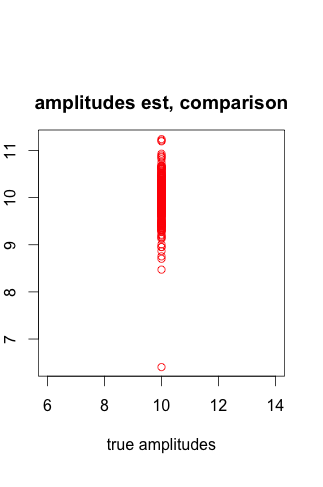
\includegraphics[height=3in]{../figures/cell_order_R_figs/amp_compare.png}
        \caption{amplitude}
    \end{subfigure}%
    ~
    \begin{subfigure}[t]{0.5\textwidth}
        \centering
        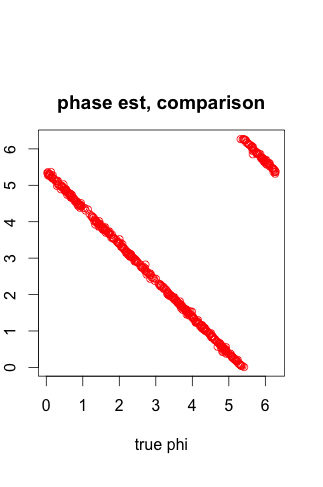
\includegraphics[height=3in]{../figures/cell_order_R_figs/phi_compare.png}
        \caption{phase}
    \end{subfigure}\\
    
     \begin{subfigure}[t]{0.5\textwidth}
        \centering
        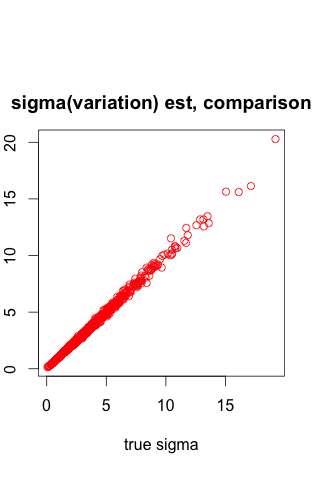
\includegraphics[height=3in]{../figures/cell_order_R_figs/sigma_compare.png}
        \caption{sigma}
    \end{subfigure}
    \caption{ The plots to compare the estimated amplitudes, phase and error variance of the genes with the true values. Ideally we would want to match the estimated values with the true values. While that seems to be fairly the case for the amplitudes and the sigma (the gene variance), it seems the results for the phase are not matching up, and looking at the linear trend in which the estimated phases are associated with the true phases, it seems the identifiability issue is making its presence felt.}
 \label{fig:fig1}
 \end{figure*}
    

\begin{figure*}[ht]
    \centering    
     \begin{subfigure}[t]{0.5\textwidth}
        \centering
        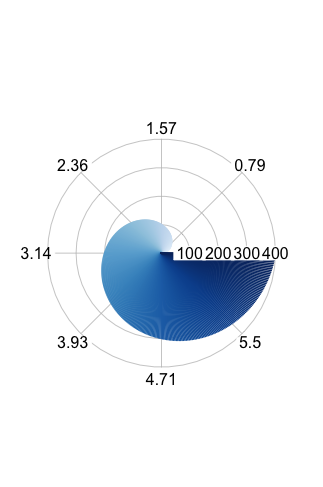
\includegraphics[height=3in]{../figures/cell_order_R_figs/original_cell_order.png}
        \caption{True radial plot}
    \end{subfigure}%
    ~
    \begin{subfigure}[t]{0.5\textwidth}
        \centering
        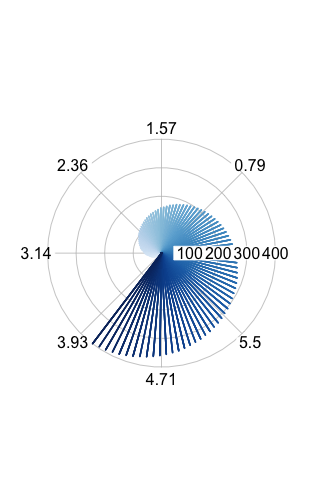
\includegraphics[height=3in]{../figures/cell_order_R_figs/estd_cell_order_100_classes.png}
        \caption{Est. radial plot - time classes}
    \end{subfigure}\\
    
     \begin{subfigure}[t]{0.5\textwidth}
        \centering
        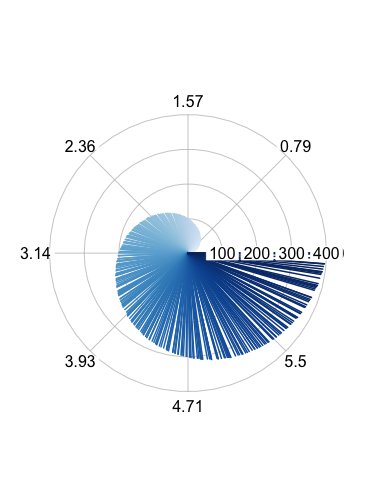
\includegraphics[height=3in]{../figures/cell_order_R_figs/estd_cell_order_phase_adjusted.png}
        \caption{Est radial plot- time, phase adjusted}
    \end{subfigure}
    \caption{We present the true and the estimated radial plots, where we put the angles in radians on the circle and then colored them in a continuous pattern from light blue  to deep blue based on the order of the observations. To make it more interpretable, we also considered the length of the angle to be proportional to the position of the cell in the full list of $400$ cells considered for simulation. The first plot (\textit{top,left}) shows the true cell cycle times of the cells. The second plot (\textit{top,right}) shows the estimated time classes with $\mathcal{T}=100$ for the cells and one can see easily that this looks more like a rotation of the first plot. The third plot (\textit{bottom}) shows the phase adjusted fully recovered estimated cell cycle times of the cells, which looks pretty similar to the true cell cycle time plot.}
 \label{fig:fig2}
 \end{figure*}

\begin{figure*}[ht]
    \centering    
     \begin{subfigure}[t]{0.5\textwidth}
        \centering
        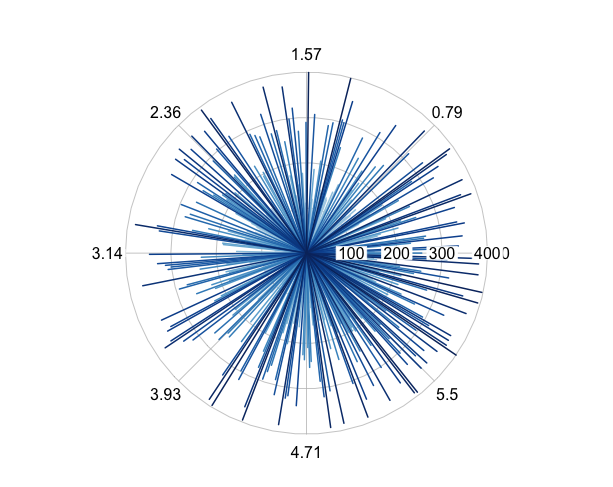
\includegraphics[height=3in]{../figures/cell_order_R_figs/original_cell_order_exp_2_unsorted.png}
        \caption{True radial plot- unsorted}
    \end{subfigure}%
    ~
    \begin{subfigure}[t]{0.5\textwidth}
        \centering
        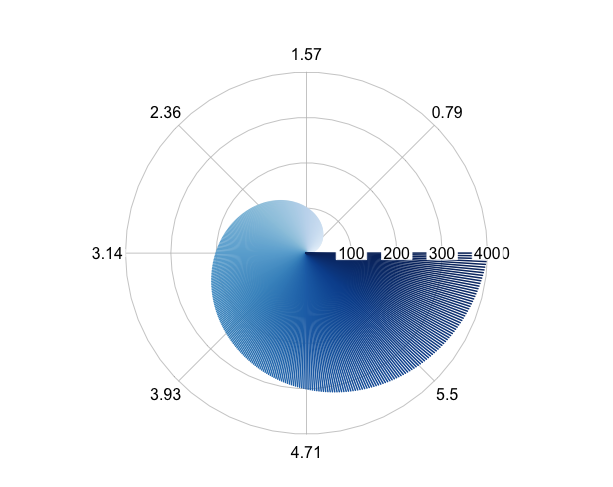
\includegraphics[height=3in]{../figures/cell_order_R_figs/original_cell_order_exp_2_sorted.png}
        \caption{True radial plot - sorted}
    \end{subfigure}\\
    
     \begin{subfigure}[t]{0.5\textwidth}
        \centering
        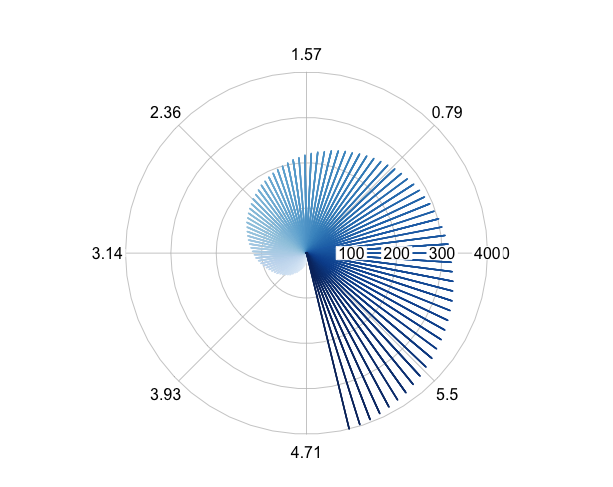
\includegraphics[height=3in]{../figures/cell_order_R_figs/estd_cell_order_100_classes_exp_2.png}
        \caption{Est radial plot- time}
    \end{subfigure}
    \caption{We present the true and the estimated radial plots, where we put the angles in radians on the circle and then colored them in a continuous pattern from light blue  to deep blue based on the order of the observations. To make it more interpretable, we also considered the length of the angle to be proportional to the position of the cell in the full list of $400$ cells considered for simulation. The first plot (\textit{top,left}) shows the true cell cycle times of the cells without sorting. The second plot (\textit{top,right}) shows the true cell cycle times in the sorted order. The third plot (\textit{bottom}) shows the estimated cell cycle order ordered as per the simulated cell cycle order. Note that the third plot almost perfectly preserves the true cell cycle order barring the rotation.}
 \label{fig:fig3}
 \end{figure*}


 \begin{figure*}[ht]
    \centering    
     \begin{subfigure}[t]{0.5\textwidth}
        \centering
        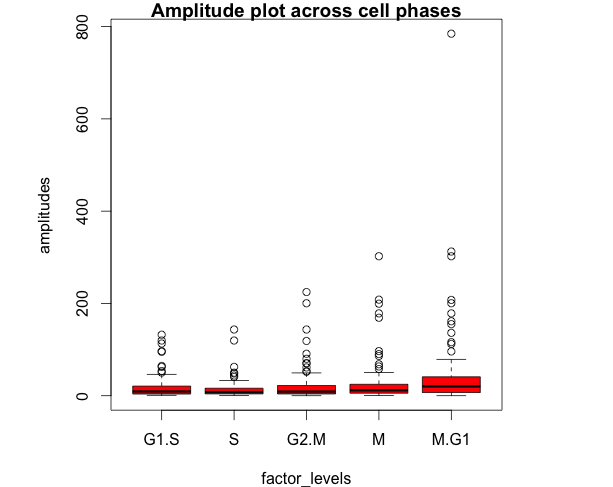
\includegraphics[height=3in]{../figures/cell_order_R_figs/amp_plot_genes_ipsc.png}
        \caption{amplitude}
    \end{subfigure}%
    ~
    \begin{subfigure}[t]{0.5\textwidth}
        \centering
        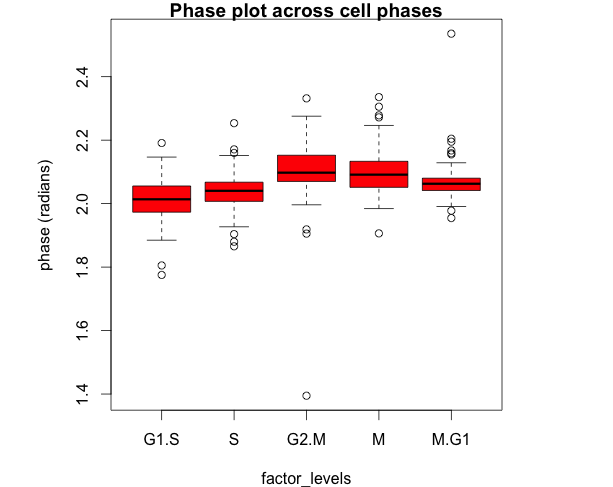
\includegraphics[height=3in]{../figures/cell_order_R_figs/phase_plot_genes_ipsc.png}
        \caption{phase}
    \end{subfigure}\\
    
     \begin{subfigure}[t]{0.5\textwidth}
        \centering
        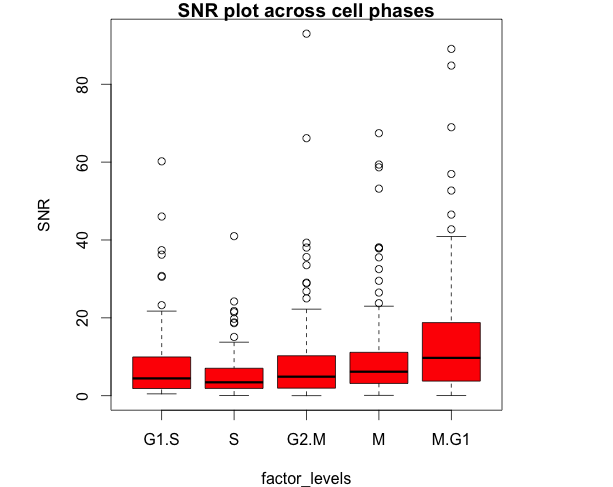
\includegraphics[height=3in]{../figures/cell_order_R_figs/snr_plot_genes_ipsc.png}
        \caption{SNR}
    \end{subfigure}
    \caption{The plots of the amplitudes, phases and SNR (signal to noise ratio) of the phase specific genes for each of the $5$ phases. The amplitudes and the SNR values do not show any notable difference, however the estimated phase distribution seems interesting. The prior belief was that it would be increasing with each phase. But it does not show such patterns. However, M and G2.M seem to be higher in phases compared to the other three phases.}
 \label{fig:fig4}
 \end{figure*}
    
 \begin{figure*}[ht]
    \centering    
     \begin{subfigure}[t]{0.5\textwidth}
        \centering
        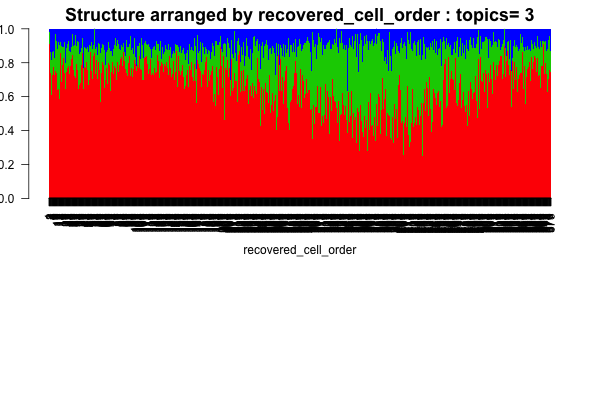
\includegraphics[height=2in]{../figures/ipsc_structure_batchcorrect_cellcycle/clus_3/struct_clus_3_recovered_cell_order.png}
        \caption{K=3, Macosko}
    \end{subfigure}%
    ~
    \begin{subfigure}[t]{0.5\textwidth}
        \centering
        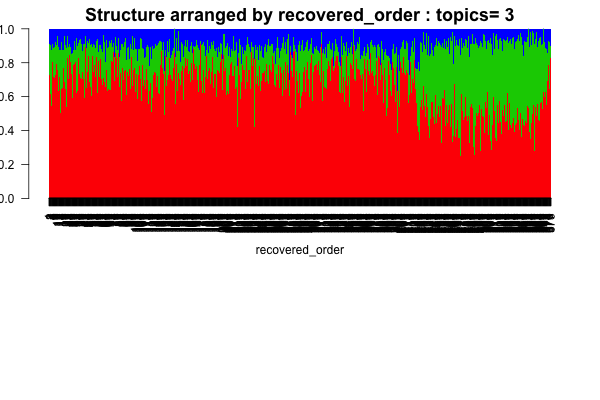
\includegraphics[height=2in]{../figures/ipsc_structure_batchcorrect_cellcycle/clus_3/struct_clus_3_recovered_order.png}
        \caption{K=3, our method}
    \end{subfigure}\\

     \begin{subfigure}[t]{0.5\textwidth}
        \centering
        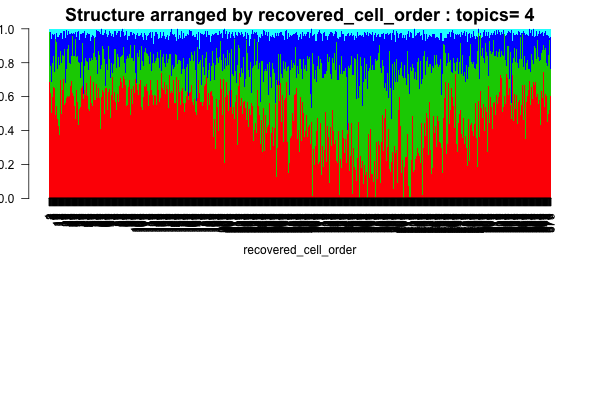
\includegraphics[height=2in]{../figures/ipsc_structure_batchcorrect_cellcycle/clus_4/struct_clus_4_recovered_cell_order.png}
        \caption{K=4, Macosko}
    \end{subfigure}%
    ~
    \begin{subfigure}[t]{0.5\textwidth}
        \centering
        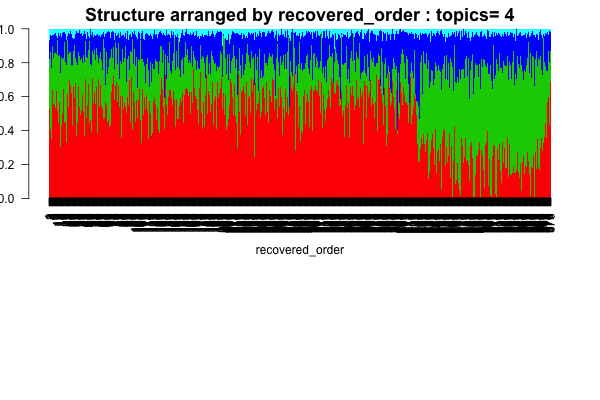
\includegraphics[height=2in]{../figures/ipsc_structure_batchcorrect_cellcycle/clus_4/struct_clus_4_recovered_order.png}
        \caption{K=4, our method}
    \end{subfigure}\\
  \caption{The admixture plots for (top) K=3 and (bottom) K=4 for the cell cycle re-ordering using Macosko method (left) and our method (right). In Macosko method, the ordering assumes that there is a montonicity in the phases from G1.S to M.G1. But, our method is more general, and it does not separate out the 5 phases, rather it seems it only separates out the M and S phases (as is true for ES cells).}
 \label{fig:fig5}
 \end{figure*}   

\subsection{Observations}

\begin{itemize}
\item The model seems to be working on the simulated models, and give us the correct ordering (as is evident from Fig \ref{fig:fig2} and Fig \ref{fig:fig3}), modulo rotation, which should be easy to fix since we have the cell phase information.

\item The application of the method on Yoav's data gives interesting results. Originally the intuition was that it would separate out the phases clearly and will explicitly show all the 5 phases G1.S, S, G2.M, M and M.G1 in the admixture plot in Fig \ref{fig:fig5}. However, this did not happen. The phases of the supposedly phase specific genes did not show the increasing order modulo $2 \pi$, which we had hoped for. One of the reasons I can think of is that since ES cells only show S and M phases, probably that is what we are seeing here only. Our method is just separating out the S and the M phases. Admixture plot in Fig \ref{fig:fig5} clearly shows two distinct patterns which mostly correlates to (M,G2.M) and (G1.S,S and M.G1) phases or more specifically, mitosis and non mitosis phases. 

\item From the admixture plots in Fig \ref{fig:fig5}., it indeed seems that our method does a better job at pooling all the mitosis phase cells together in a more homogeneous compared to Macosko's method (the proportion of green cluster is more homogeneous in our case than in Macosko's case). 

\item I repeated the experiment taking only high SNR (SNR $>$ 10) genes so that I can keep the noisy genes away and ensuring that they do not screw up the analysis. This gave us $277$ genes satisfying the above SNR condition (which is pretty high actually). When we observed the patterns on these genes only, I got a very similar looking admixture plot in Fig \ref{fig:fig5} (that is why did not present it here but I have it saved in my laptop). This indeed suggests that the genes which only account for noise are not really effecting the analysis as much.

\item I am not sure but it may happen that the phase specific genes were obtained from non iPSC cells, where the phases were clearly visible and which has arrest phases and longer phases. So, may be that is one reason why the genes are not really showing the 5 phases for our case?

\end{itemize}


\subsection{Road Ahead}

\begin{itemize}

\item Make sense of the observations.....what is the story here?

%\item To fix the identifiability issue in a meaningful way, possibly pooling in information from phase specific cell cycle genes. Would probably be worthwhile to think about  whether we can fix this without relying on cell cycle genes so much, as the identification of these phase specific genes may not be foolproof.

%\item To implement the Bayesian version, which should not be very difficult. We may think about what priors we want to set though. I am more interested in having a meaningful prior for phases that takes into account the cell cycle gene information, thereby fixing identifiability. 

\item To see if we can build a classifier from the phase distribution of the genes in the different phases (which was actually found to be different in different phases and may be a good yardstick for classification).

\item To speed up the code : currently the $578$ samples and $543$ genes case takes around $20$ minutes to run and converge (at tolerance 0.1) of the log-likelihood which happens pretty quickly around $30-40$ iterations. Need to speak with Raman about one part of the code which seems to be the only time expensive component.
\end{itemize}




\section{Discussion}

\subsection{Why sinusoidal and not Fourier}

One suggestion we were discussing recently in the context that the gene expression curved did not look very sinusoidal was to use  a sum of sinusoids (which is basically Fourier) or a mixture of sinusoids (which I think will be analogous to sum of sinusoids as we will not be able to separate out the mixing proportions and the amplitudes of the individual components due to lack of identifiability). I think this will not really make a difference because in that case, we shall assume 

$$ Y_{sg} = \sum_{l=1}^{L} \alpha_{lg} sin (t_s + \phi_{lg})  +\epsilon_{sg}, \hspace{1 in}  \epsilon_{sg} \sim N(0, \sigma^2_j)  $$

Note that we keep the frequency of each sinusoid 1, because firstly, I guess we want them to have period $2 \pi$ as we are looking at the state space which is a circle for the cell cycle. The other reason is computational. If we have a frequency for each sinusoid, say $\omega_{lg}$, then we have serious lack of identifiability. We can write $\omega^{'}_{lg} = \omega_{lg} \times 100$ for all $l$ and $g$ and $t^{'}_s = t_s/100$ for all $s$ and the model remains the same. I do not know of any good prior that can handle such a scenario.

In that case, we can write the total loglikelihood as 

$$ \mathcal{L} \sim  \propto \prod_{s=1}^{S} \prod_{g=1}^{G} N ( \sum_{l=1}^{L}  \alpha_{lg} sin (t_s + \phi_{lg}), \sigma^2_{g} ) $$

or we can write 

\begin{align*}
Y_{sg}  & =  \sum_{l=1}^{L}  \alpha_{lg} sin (t_s + \phi_{lg}) + \epsilon_{sg}  \\
	    & = sin(t_s) \sum_{l=1}^{L} \alpha_{lg} cos(\phi_{lg}) + cos(t_s) \sum_{l=1}^{L} \alpha_{lg} sin(\phi_{lg}) + \epsilon_{sg}\\
	    & = \beta_{1g} sin(t_s) + \beta_{2g} cos(t_s)  + \epsilon_{sg}\\
	    & =  \lambda_g sin (t_s + \nu_g)  + \epsilon_{sg}\\
\end{align*}

where 

$$ \lambda_{g} = \sqrt{\beta^2_{1g} +  \beta^2_{2g}} $$

$$ \nu_g = tan^{-1}  \left (\frac{\beta_{2g}}{\beta_{1g}} \right ) $$   

So basically with the frequencies across the sinusoids remaining the same, we are ultimately getting a sinusoid only it seems (if my calculations are correct). That is taking us back to the previous assumption we had. 

\subsection{Cell phase length}

One of the important considerations has been how should we move from the  time classes to actual  cell cycle phases - G1, S, G2.M, M and M.G1. Originally the idea was to split up the cell cycle appropriately and assign the partitions to these cell phases. However, the task is pretty difficult from biological standpoint. For a typical rapidly proliferating human cell with a total cycle time of $24$ hours, the G1 phase lasts around $11$ hours, S phase lasts about $8$ hours, G2 about $4$ hours and M about 1 hour. So, the partitioning is definitely not uniform across the cell phases. To further complicate matters in embryonic stem cells which are very rapidly proliferating, cell cycles are about 30 minutes long with just the S phase and the M phase (minimal growth phases observed). There is also the possibility that a cell in a G1 phase may hit an energy barrier and stop growing due to lack of nutrients or extracellular impulse and enter a quiescent phase called G0, and stay there until it gets activated by enzymes to overcome the barrier. So, overall, the moral of the story is that it is nearly impossible to deduce the cell phases merely looking at the relative ordering of the cells or their position on the cycle. This is where, it is vital that we pool in information from the cell cycle phase specific genes in order to assign these cells into different cell phases. Also, it makes it very difficult to assign a particular phase value for these phase specific genes, because assigning a phase value will require one to have information about the phase lengths of each phase, which is difficult to track down. 

\subsection{Problem of identifiability}

If we do not constrain the phases, the model no longer remains identifiable. One can just take 

$$ t^{'}_s = t_{s} + \epsilon \hspace{1 in} \forall s $$
$$ \phi^{'}_{g} = \phi_{g} - \epsilon \hspace{1 in} \forall g $$

As a result of this, we may get estimated phases and estimated cell times that are shifted. If we do not have prior information about relative order of the phases or the relative order of the cell times, then it will be difficult to extract the correct estimates of $t$ and $\phi$ and what we would end up estimating is a rotation of the actual time points. To solve this problem, again we may need to use the phase specific genes expression to drive the knowledge of a broad order among the cells, which can give us the suitable anti-rotation to get the back estimates of the original times.





\end{document}




